%!TEX root = report.tex
Note that we have used the Xtion to complete this exercise, instead of the provided bag file.\\

For this exercise we have defined a package called \t{basics}. In this package we have created a folder \t{launch}, in which we placed the launch file presented presented in \cref{lst:1:launchFile}.

\lstinputlisting[caption={The launch file for the camera, \t{camera.launch}.}, label={lst:1:launchFile}, language=XML]{./src/1/camera.launch}

The tag \xml{<launch>} is the root element of the file \t{camera.launch}, it indicates that we are defining a launch file. Launch files allow us to start multiple nodes at once. The child tag \xml{<node>}, of \xml{<launch>} indicates which ROS node we would like to launch. The attributes \xml{pkg} and \xml{type}, the name of the executable,  attribute identify which program ROS should run to start this node. The attribute \xml{name} assigns a name to the node. 

We use a \t{static_transform_publisher} which publishes a static coordinate transform. This executable requires several arguments, which are passed via the attribute \xml{args}. One should call the \t{static_transform_publisher} as follows
\begin{lstlisting}[language=XML]
	static_transform_publisher x y z yaw pitch roll frame_id child_frame_id period_in_ms
\end{lstlisting}
The \xml{x}, \xml{y}, \xml{z} indicate an offset in the $x$, $y$ and $z$-direction. We have used a $z$ offset of \SI{1.4}{\meter} to correct for the height of the stand of the Xtion. The $x$ and $y$ offset ensure that the frame is placed in the middle of the point cloud, presented in \cref{fig:1:finalResult}. 

The \xml{yaw}, \xml{pitch} and \xml{roll} define the rotation around respectively the $z$, $y$ and $x$ axis in radians. The pitch \SI{0.72}{\radian} corrects for the angle of the Xtion, which translates to around $\rfrac{1}{4}\pi$. The \xml{yaw} and \xml{roll} should be zero in a perfectly calibrated stand, however we needed to tweak the roll a bit to get the point cloud were we wanted it, due to the camera not being perfectly parallel to the floor. 

\begin{figure}
	\centering
	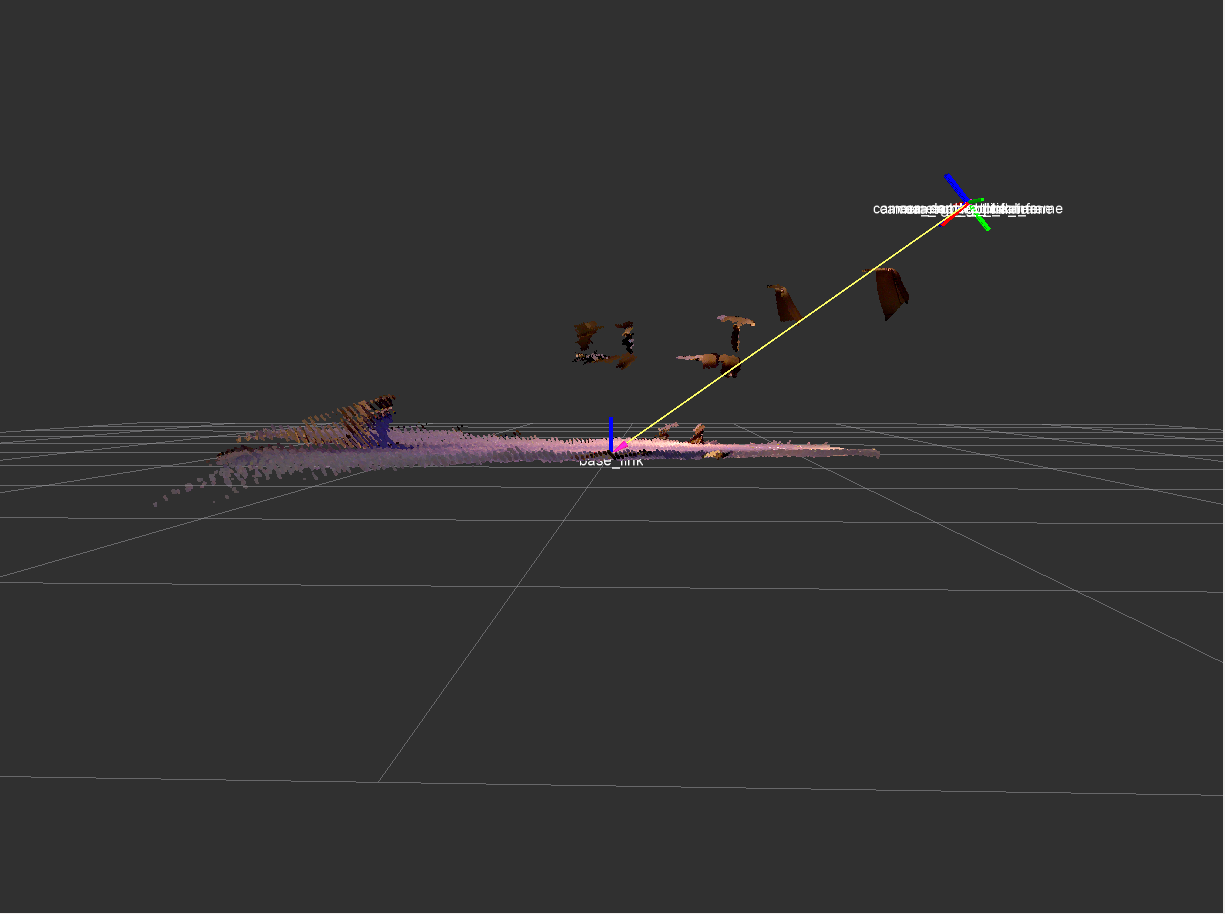
\includegraphics[width=0.48\textwidth]{./img/Assignment1_1}
	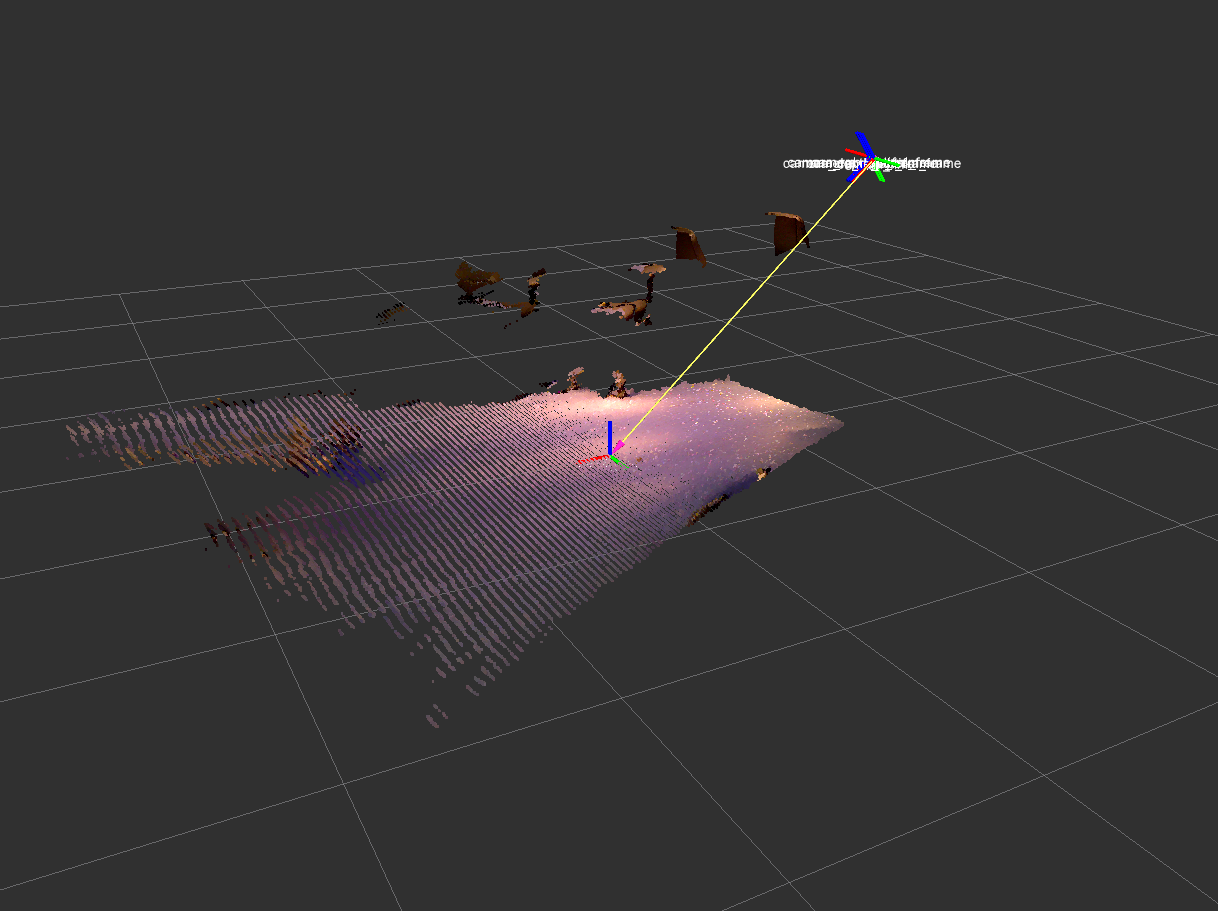
\includegraphics[width=0.48\textwidth]{./img/Assignment1_2}	
	\caption{The point as visualized by \t{rviz}, under two different angles, after the application of the static transformation defined in \cref{lst:1:launchFile}.}
	\label{fig:1:finalResult}
\end{figure}


Following the earlier mentioned information there are two values, which are  \xml{frame_id} and \xml{child_frame_id}. These refer to the link and its parent link. In our model they are the base link and the camera link, respectively. The camera link shows the base point from which the camera records the information it receives, and the base link works as a reference point for the floor in the case of the information that we received. This can be seen in Figure \ref{fig:1:finalResult} . The yellow line shows the link between the base link and the camera link.

We have set \xml{period_in_ms} to \SI{100}{\milli\second}, which is the value recommended by the ROS documentation. 

% We have launched the camer with the following command: \t{roslaunch openni2_launch openni2.launch}.
